\chapter{Aanpassingen van planten en fenotypische plasticiteit}\label{ch:b2:plant-plasticity}

Twee bladeren van dezelfde eik: dat van de top van de kroon is klein, dik
en leerachtig, dat uit het beschaduwde binnenste drie keer zo groot en zo
dun als papier. Een zaailing van dezelfde eik onder een gesloten bladerdak
groeit hoog en spichtig op; zijn broertje op een open plek blijft kort en
stevig. Geen van beide verschillen is genetisch. Een plant kan niet naar
een betere plek lopen, dus bouwt ze zich zo dat ze past bij de plek die ze
heeft: ze neemt licht, zwaartekracht, aanraking, water, zout en kou waar, en
buigt, verdikt, strekt zich, sluit haar poriën of verhardt haar cellen
naargelang. Dit hoofdstuk gaat over die plasticiteit --- hoe een plant haar
omgeving afleest en wat ze eraan doet --- en over de erfelijke aanpassingen
waarmee plantenlijnen zich hebben aangepast aan woestijnen, schaduw, zout en
vorst.

\section{Plasticiteit en haar grenzen}

\begin{definition}[Fenotypische plasticiteit en de reactienorm]\label{def:b2:plant-plasticity:plasticity}
\index{fenotypische plasticiteit}\index{reactienorm}\index{acclimatisatie}\index{adaptatie}
\emph{Fenotypische plasticiteit} is het vermogen van één \omterm{def:b2:meiosis-heredity:vocabulary}{genotype} om in
verschillende omgevingen verschillende \omterm{def:b2:meiosis-heredity:vocabulary}{fenotypen} voort te brengen. De
\emph{reactienorm} van een \omterm{def:b2:meiosis-heredity:vocabulary}{genotype} is de kromme van zijn \omterm{def:b2:meiosis-heredity:vocabulary}{fenotype} tegen een
omgevingsvariabele --- bladdikte tegen licht, stengellengte tegen
temperatuur; \omterm{def:b2:meiosis-heredity:vocabulary}{genotypen} verschillen in hun reactienormen, en die verschillen
zijn erfelijk, ook wanneer de plasticiteit zelf dat niet is.
\emph{Acclimatisatie} is de omkeerbare, fysiologische vorm: een blad dat in
een droge week zijn cuticula verdikt, een cel die in de herfst
antivries maakt. \emph{Adaptatie}, in evolutionaire zin, is de erfelijke
afstemming van een lijn op haar habitat, over generaties geselecteerd; een
cactus is aangepast aan droogte, een boon acclimatiseert aan een droge
periode. Planten zijn plastischer dan dieren omdat ze modulair en
onbegrensd zijn (\cref{ch:b2:plant-meristems}): het volgende blad kan anders
worden gebouwd dan het vorige, en het sessiele bestaan maakt plasticiteit de
enige manier om te bewegen.
\end{definition}

\begin{omfigure}
\begin{tikzpicture}
\begin{axis}[
  width=0.72\linewidth, height=5.4cm,
  axis x line=bottom, axis y line=left,
  xmin=0, xmax=100, ymin=0, ymax=1.2,
  xlabel={licht (\% van de volle zon)}, ylabel={bladdikte (relatief)},
  xlabel style={font=\small, at={(axis description cs:0.5,-0.13)}, anchor=north},
  ylabel style={font=\small},
  tick label style={font=\small}, xtick={0,25,50,75,100}, ytick={0,0.5,1},
  legend style={font=\scriptsize, at={(0.97,0.08)}, anchor=south east, draw=none},
  clip=false,
]
\addplot[very thick, omDef, domain=2:100, samples=60] {0.35 + 0.65*(1-exp(-x/30))};
\addlegendentry{genotype 1: een plastische eik}
\addplot[very thick, omThm, domain=2:100, samples=60] {0.55 + 0.2*(1-exp(-x/30))};
\addlegendentry{genotype 2: een minder plastische}
\end{axis}
\end{tikzpicture}

{\small Twee \omterm{def:b2:plant-plasticity:plasticity}{reactienormen}. Elk \omterm{def:b2:meiosis-heredity:vocabulary}{genotype} maakt dikkere bladeren bij meer
licht; de helling van de kromme --- de plasticiteit --- is zelf een erfelijk
kenmerk, en de twee \omterm{def:b2:meiosis-heredity:vocabulary}{genotypen} verschillen erin.}
\end{omfigure}

\begin{proposition}[Zonnebladeren en schaduwbladeren]\label{prop:b2:plant-plasticity:sunshade}
\index{zonneblad}\index{schaduwblad}
Een blad dat zich in de volle zon ontwikkelt, is klein en dik, met twee of
drie lagen palissadecellen, veel huidmondjes, een dikke cuticula, een hoge
concentratie van het koolstoffixerende enzym en een hoge maximale
fotosynthesesnelheid; een blad van dezelfde plant dat zich in de schaduw
ontwikkelt, is groot en dun, met één palissadelaag, meer chlorofyl per
massa-eenheid, een lage ademhalingssnelheid en een laag
lichtcompensatiepunt. Het \omterm{prop:b2:plant-plasticity:sunshade}{schaduwblad} is gebouwd om elk foton tegen minimale
kosten te oogsten, het \omterm{prop:b2:plant-plasticity:sunshade}{zonneblad} om een vloed ervan te benutten zonder
oververhit te raken of te verwelken. De beslissing valt terwijl het blad nog
een primordium is, op grond van het licht --- en in het bijzonder de kleur
ervan --- dat de knop bereikt; een volgroeid blad kan zichzelf niet
herbouwen, en daarom verbrandt een plant die van de schaduw naar de zon
wordt verplaatst tot ze nieuwe bladeren heeft gemaakt.
\end{proposition}

\begin{omfigure}
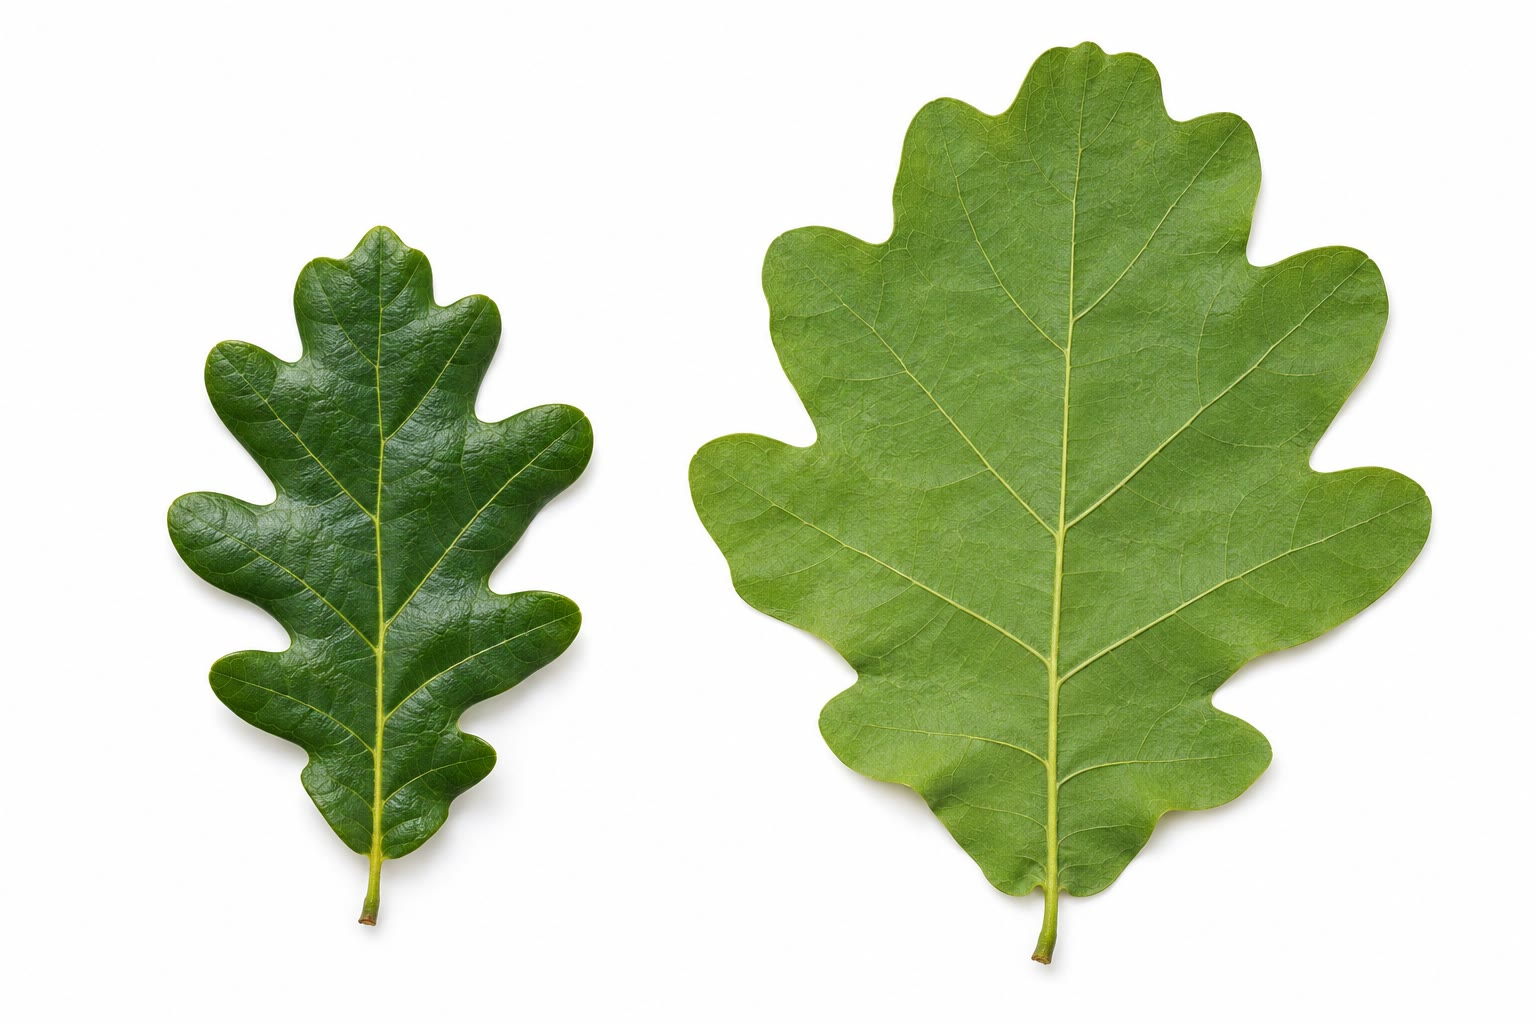
\includegraphics[width=0.55\linewidth]{images/book4/ai/b4-15-sun-shade-leaves.jpg}

{\small Een \omterm{prop:b2:plant-plasticity:sunshade}{zonneblad} en een \omterm{prop:b2:plant-plasticity:sunshade}{schaduwblad} van één eik: hetzelfde \omterm{def:b2:meiosis-heredity:vocabulary}{genotype},
ander licht, andere bladeren.}
\end{omfigure}

\section{Het licht aflezen}

\begin{theorem}[Fytochroom als meter van de lichtkwaliteit]\label{thm:b2:plant-plasticity:phytochrome}
\index{fytochroom}\index{rood-verroodverhouding}\index{schaduwvermijding}
Fytochroom bestaat in twee vormen: $P_r$, dat rood licht (\qty{660}{nm})
absorbeert en wordt omgezet in $P_{fr}$, en $P_{fr}$, dat verrood
(\qty{730}{nm}) absorbeert en wordt teruggezet --- en het is
$P_{fr}$ dat werkt. In continu licht houden de twee omzettingen elkaar in
evenwicht in een \emph{fotoevenwicht} waarvan de ligging alleen afhangt van
de verhouding van rood tot verrood in het licht:
\[
\varphi = \frac{P_{fr}}{P_{r} + P_{fr}} = \frac{R}{R + a\,FR},
\]
waarin $R$ en $FR$ de fotonfluxdichtheden in de twee banden zijn
en $a$ een constante van het pigment ($a \approx 0.77$). Zonlicht heeft
$R{:}FR \approx 1.15$, wat $\varphi \approx 0.6$ geeft; licht dat door
bladeren is gefilterd, die rood absorberen en verrood doorlaten, heeft
$R{:}FR
\approx 0.2$ en $\varphi \approx 0.2$. Een lage $\varphi$ vertelt een plant
dat ze onder of naast andere planten staat, nog voordat ze werkelijk wordt
beschaduwd --- verrood dat door een buur wordt teruggekaatst, wordt aan de
kant die naar die buur is gekeerd waargenomen --- en ze reageert met het
\emph{schaduwvermijdingssyndroom}: snellere strekking van de stengel,
langere bladstelen, omhoog gehouden bladeren, minder vertakking, vroegere
bloei. Een zaailing onder een gesloten bladerdak verdubbelt zijn
strekkingssnelheid.
\end{theorem}
\begin{proof}
Zij $k_1 R$ de snelheidsconstante voor $P_r \to P_{fr}$ (evenredig met de
rode flux) en $k_2\,FR$ die voor $P_{fr} \to P_r$. In evenwicht is
$k_1 R\,P_r = k_2\,FR\,P_{fr}$, dus $P_{fr}/P_r = k_1 R/
(k_2 FR)$ en $\varphi = P_{fr}/(P_r + P_{fr}) = R/(R + a\,FR)$ met
$a = k_2/k_1$. (Beide vormen absorberen enigszins in beide banden, wat de
constante $a$ opvangt; de vorm van het resultaat blijft dezelfde.) Met
$a = 0.77$: $1.15/(1.15 + 0.77) = 0.60$; $0.2/(0.2 + 0.77) = 0.21$.
\end{proof}

\begin{omfigure}
\begin{tikzpicture}
\begin{axis}[
  width=0.7\linewidth, height=5.2cm,
  axis x line=bottom, axis y line=left,
  xmin=0, xmax=1.4, ymin=0, ymax=0.8,
  xlabel={verhouding rood : verrood van het licht}, ylabel={$\varphi = P_{fr}/P_{\text{totaal}}$},
  xlabel style={font=\small, at={(axis description cs:0.5,-0.13)}, anchor=north},
  ylabel style={font=\small},
  tick label style={font=\small}, xtick={0,0.2,0.6,1.15}, ytick={0,0.2,0.4,0.6},
  clip=false,
]
\addplot[very thick, omDef, domain=0:1.4, samples=60] {x/(x+0.77)};
\draw[dashed, gray] (axis cs:1.15,0) -- (axis cs:1.15,0.6) -- (axis cs:0,0.6); \node[font=\scriptsize, anchor=south west] at (axis cs:1.15,0.6) {volle zon};
\draw[dashed, gray] (axis cs:0.2,0) -- (axis cs:0.2,0.21) -- (axis cs:0,0.21); \node[font=\scriptsize, anchor=west] at (axis cs:0.25,0.15) {onder een bladerdak};
\end{axis}
\end{tikzpicture}

{\small Het fotoevenwicht van fytochroom tegen de verhouding van rood tot
verrood. Zonlicht houdt het grootste deel van het pigment in de actieve
vorm; door bladeren gefilterd licht houdt het grotendeels inactief, en de
plant leest het verschil als buren.}
\end{omfigure}

\begin{proposition}[Fototropie]\label{prop:b2:plant-plasticity:phototropism}
\index{fototropie}\index{tropie}\index{hypothese van Cholodny--Went}
Een \emph{tropie} is een groeibeweging die door een gerichte prikkel wordt
georiënteerd. Bij \emph{fototropie} buigt een scheut naar blauw licht toe:
het licht wordt in de top waargenomen door een blauwlichtreceptor
(fototropine), de auxine die uit de top neerdaalt, wordt naar de
beschaduwde kant omgeleid --- de dragers ervan verplaatsen zich naar het
laterale membraan --- en de beschaduwde kant, die meer auxine krijgt,
strekt zich sneller dan de belichte kant, zodat de scheut naar het licht
toe kromt. Het buigen is ongelijke groei, geen spier: het gebeurt alleen in
de strekkingszone, duurt een of twee uur en is onomkeerbaar. Wortels,
waarin hetzelfde overschot aan auxine de strekking juist \emph{remt},
buigen ervan weg.
\end{proposition}
\begin{proof}[Bewijsmateriaal]
Darwin (1880) toonde met coleoptielen van grassen aan dat de top het licht
waarneemt en de zone eronder buigt: het afdekken van de top met een
ondoorzichtig kapje hief het buigen op, het afdekken van de basis met een
kokertje niet, en een doorzichtig kapje liet het intact. Boysen-Jensen
(1913) sneed de top af en zette hem terug met een blokje gelatine ertussen:
het buigen bleef, dus was het signaal een diffundeerbare stof; een plaatje
mica aan de beschaduwde kant blokkeerde het, aan de belichte kant niet, dus
reisde de stof langs de beschaduwde kant naar beneden. Went (1928) ving de
stof op in agar uit afgesneden toppen en vond dat een blokje dat
excentrisch op een onthoofde coleoptiel in het donker werd geplaatst, die
van het blokje weg liet buigen --- onder een hoek evenredig met de
hoeveelheid --- en toen hij agar verzamelde uit de twee helften van een
eenzijdig belichte top, vond hij ongeveer twee derde van de auxine aan de
beschaduwde kant en een derde aan de belichte kant (Briggs, 1957, met
betere methoden). De laterale herverdeling van een groeihormoon is de
\omterm{prop:b2:plant-plasticity:phototropism}{hypothese van Cholodny en Went}, en die heeft standgehouden.
\end{proof}

\begin{omfigure}
\begin{tikzpicture}[every node/.style={font=\scriptsize}, >=stealth]
  \foreach \x/\lab/\cap/\bend in {0/{intact:\\buigt}/0/1, 2.6/{top afgedekt:\\geen buiging}/1/0, 5.2/{basis afgedekt:\\buigt}/2/1, 7.8/{top afgesneden:\\geen buiging}/3/0, 10.4/{top op gelatine:\\buigt}/4/1} {
    \begin{scope}[xshift=\x cm]
      \fill[omExo!30] (-0.7,0) rectangle (0.7,0.2);
      \ifnum\bend=1
        \draw[very thick, omExo!70!black] (0,0.2) -- (0,1.6) .. controls (0,2.3) and (0.5,2.6) .. (0.9,2.8);
      \else
        \draw[very thick, omExo!70!black] (0,0.2) -- (0,3.0);
      \fi
      \ifnum\cap=1 \fill[black] (-0.2,2.7) rectangle (0.2,3.1); \fi
      \ifnum\cap=2 \fill[black] (-0.2,0.2) rectangle (0.2,1.5); \fi
      \ifnum\cap=3 \draw[thick] (-0.3,2.6) -- (0.3,2.6); \fi
      \ifnum\cap=4 \fill[omDef!35] (-0.2,2.55) rectangle (0.2,2.75); \draw[very thick, omExo!70!black] (0.55,2.75) -- (0.9,3.1); \fi
      \node[below, align=center] at (0,-0.15) {\lab};
    \end{scope}
  }
  \node[anchor=east, align=right, omProp!80!black] at (-1.0,2.2) {licht van\\rechts $\to$};
\end{tikzpicture}

{\small De proeven met coleoptielen. Darwin: de top neemt het licht waar en
het gebied eronder buigt; de top afdekken houdt het tegen, de basis
afschermen niet. Boysen-Jensen: het signaal steekt een blokje gelatine over
--- het is een stof.}
\end{omfigure}

\begin{omfigure}
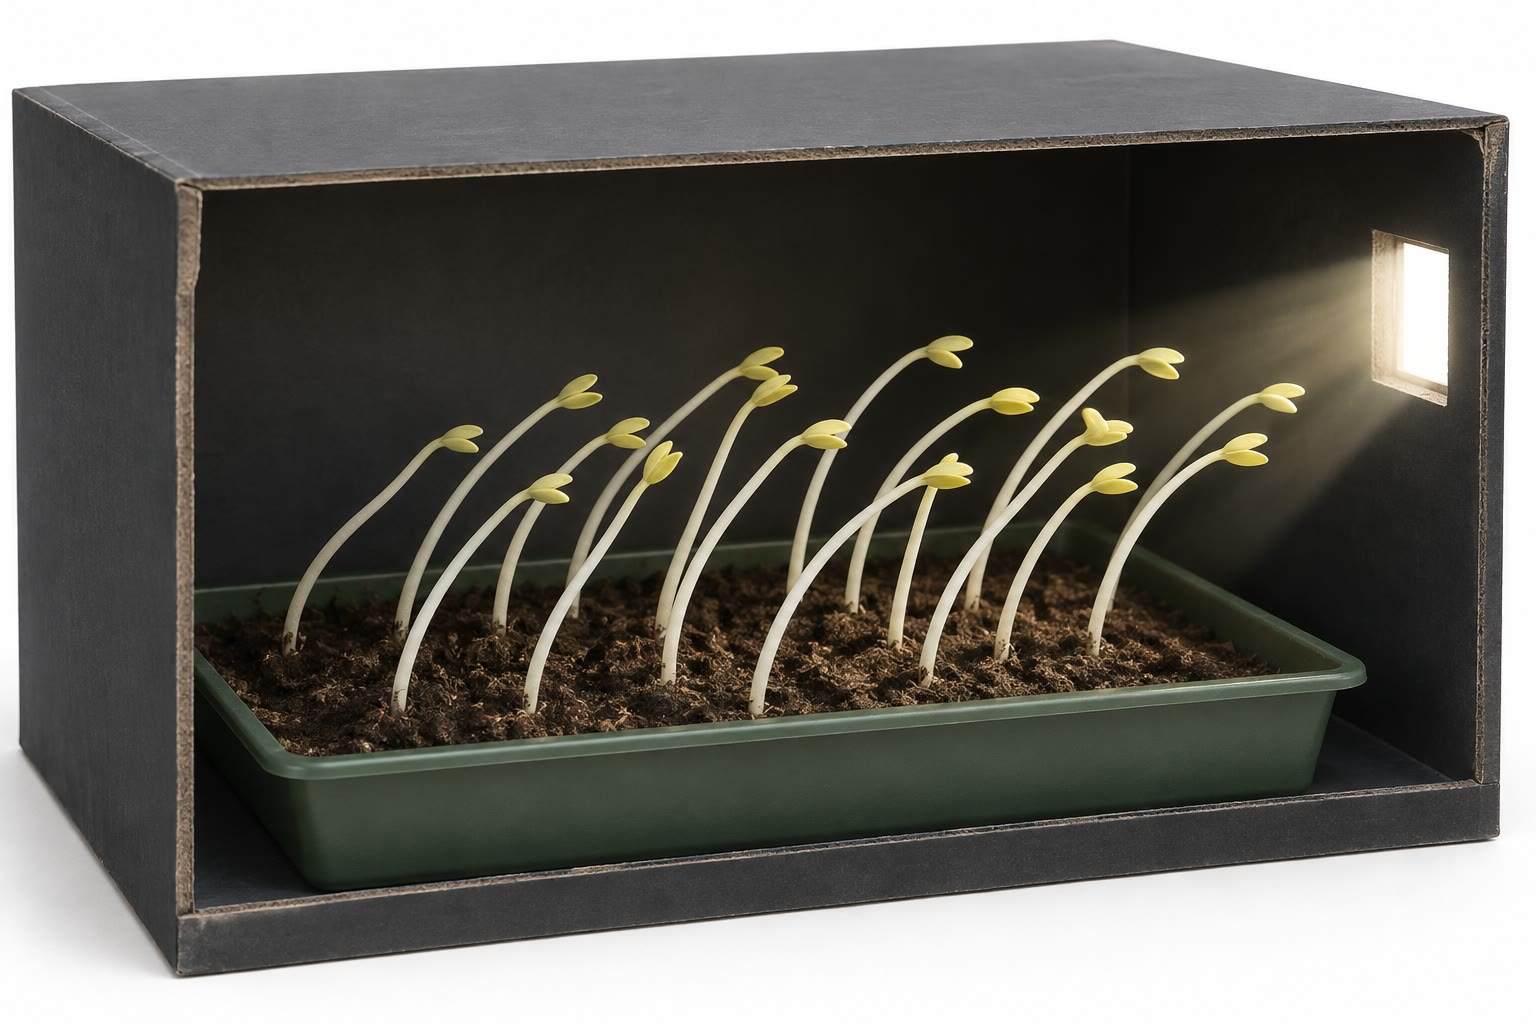
\includegraphics[width=0.55\linewidth]{images/book4/ai/b4-15-phototropism.jpg}

{\small Zaailingen in een doos met één raam: allemaal buigen ze naar het
licht, door aan de kant die ervan is afgekeerd sneller te groeien.}
\end{omfigure}

\begin{theorem}[Hoeveel een stengel buigt]\label{thm:b2:plant-plasticity:bend}
Als de beschaduwde kant van een stengel met diameter $d$ zich met een
relatieve hoeveelheid $\varepsilon_s$ strekt en de belichte kant met
$\varepsilon_l$, over een groeizone met lengte $L$, kromt de zone over een
hoek
\[
\theta = \frac{L\,(\varepsilon_s - \varepsilon_l)}{d}
\]
(in radialen). Een coleoptiel die met \qty{5}{\%} per uur groeit over een
zone van \qty{10}{mm} en \qty{1}{mm} dik is, met auxine verdeeld als
$65 : 35$, zodat de twee kanten met $1.3$ en $0.7$ keer het gemiddelde
groeien, buigt in drie uur over $\theta = 10\times(0.195 - 0.105)/1 =
0.9$ radialen, ongeveer \qty{50}{\degree}. Buigen vraagt geen nieuw
mechanisme: de gewone groei van \cref{ch:b2:plant-meristems}, aan twee
kanten ongelijk gemaakt, volstaat.
\end{theorem}
\begin{proof}
De twee kanten van de zone worden bogen met stralen $\rho + d/2$ en
$\rho - d/2$ die dezelfde hoek $\theta$ insluiten, met lengten $L(1 +
\varepsilon_s)$ en $L(1 + \varepsilon_l)$; hun verschil is
$\theta d$, dus $\theta = L(\varepsilon_s - \varepsilon_l)/d$. Over
drie uur bij \qty{5}{\%} per uur is de gemiddelde verlenging $0.15$;
$1.3\times 0.15 = 0.195$ en $0.7\times 0.15 = 0.105$.
\end{proof}

\begin{proposition}[Gravitropie]\label{prop:b2:plant-plasticity:gravitropism}
\index{gravitropie}\index{statoliet}
Een scheut die op zijn zij wordt gelegd, draait binnen enkele uren omhoog en
een wortel omlaag. De richting van de zwaartekracht wordt waargenomen door
\emph{statolieten} --- zware zetmeelkorrels in gespecialiseerde cellen van
het wortelmutsje en van de zetmeelschede van de stengel --- die in seconden
naar de onderkant van de cel zakken en, door op het membraan of het
endoplasmatisch reticulum te drukken, de auxinedragers omleiden, zodat
auxine zich aan de onderkant ophoopt. In de scheut groeit de onderkant
sneller en kromt de stengel omhoog; in de wortel remt hetzelfde overschot
aan auxine de onderkant, groeit de bovenkant sneller en kromt de wortel
omlaag. Verwijder het wortelmutsje en de wortel groeit recht in elke
richting; zetmeelloze mutanten nemen de zwaartekracht slecht waar; een
wortel op een langzaam draaiende trommel (een klinostaat), die de
statolieten nooit laat zakken, groeit zonder richting. De respons is een
tweede toepassing van het mechanisme van Cholodny en Went, met een andere
sensor.
\end{proposition}

\section{Water: de poriën sluiten}

\begin{proposition}[Regeling van de huidmondjes]\label{prop:b2:plant-plasticity:stomata}
\index{huidmondje}\index{sluitcel}\index{abscisinezuur}\index{stomatale geleidbaarheid}
De poriën van het blad, de \emph{huidmondjes}, worden elk begrensd door twee
\emph{sluitcellen} waarvan de wanden ongelijk verdikt zijn, zodat ze, wanneer
ze kalium en water opnemen en opzwellen, uit elkaar buigen en de porie
openen, en wanneer ze die verliezen, haar sluiten. Ze gaan 's ochtends open
onder blauw licht en een laag inwendig $\mathrm{CO_2}$, en sluiten in het
donker; ze sluiten binnen enkele minuten wanneer er \emph{\omterm{def:b2:plant-flowering:dormancy}{abscisinezuur}}
aankomt --- gemaakt in wortels die uitdrogende grond waarnemen en via het
xyleem omhoog gevoerd, of in het blad zelf gemaakt wanneer het turgor
verliest --- en wanneer de lucht erg droog is. De \emph{\omterm{prop:b2:plant-plasticity:stomata}{stomatale
geleidbaarheid}} $g_s$ bepaalt zowel het verloren water,
$E = g_s\,(w_i - w_a)$ (het verschil in molfractie waterdamp tussen het
verzadigde inwendige van het blad en de lucht), als het opgenomen
$\mathrm{CO_2}$, $A = g_s\,(c_a -
c_i)/1.6$ (de factor $1.6$ is de verhouding van de diffusiecoëfficiënten
van waterdamp en $\mathrm{CO_2}$). Het blad ruilt water voor koolstof via
één klep, en zijn \emph{watergebruiksefficiëntie} is
\[
\frac{A}{E} = \frac{c_a - c_i}{1.6\,(w_i - w_a)},
\]
enkele duizendsten mol koolstof per mol water: een typisch C$_3$-blad
besteedt \qtyrange{400}{600}{g} water per gram vastgelegde koolstof, een
C$_4$-blad de helft daarvan, een \omterm{prop:b2:plant-plasticity:xerophytes}{CAM-plant} een vijfde.
\end{proposition}

\begin{omfigure}
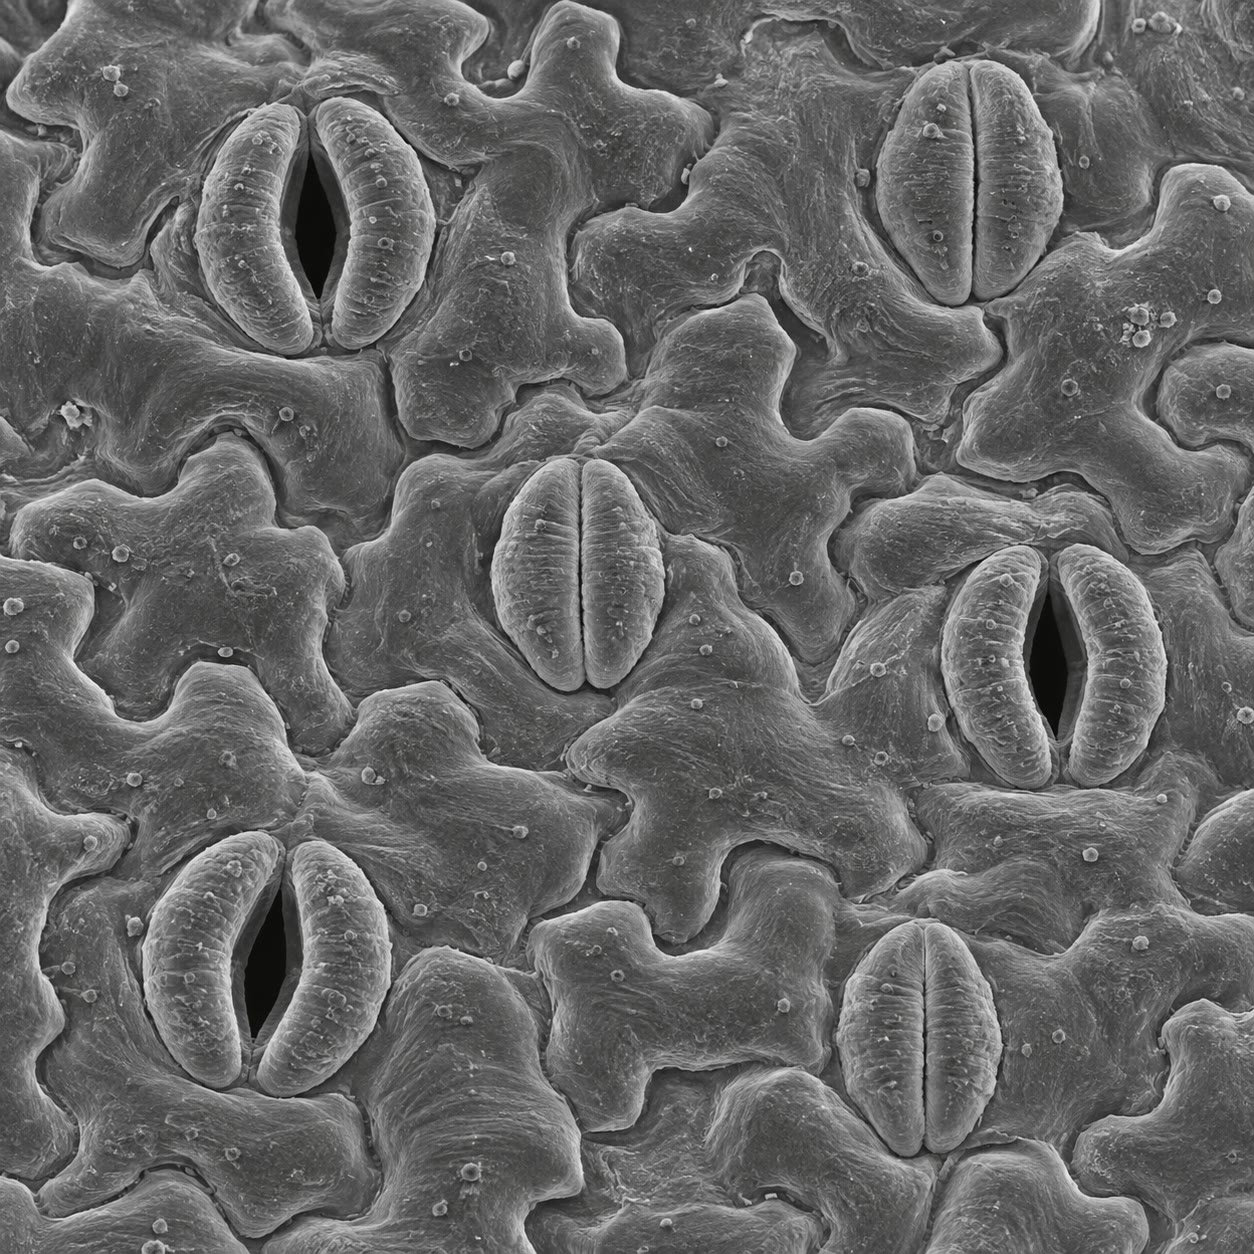
\includegraphics[width=0.42\linewidth]{images/book4/ai/b4-15-stomata-sem.jpg}

{\small Huidmondjes aan de onderkant van een blad, sommige open en sommige
gesloten: twee sluitcellen rond elke porie, de klep waarlangs het blad water
ruilt voor koolstofdioxide.}
\end{omfigure}

\begin{example}[De prijs van de koolstof van een dag]\label{ex:b2:plant-plasticity:wue}
Op het middaguur transpireert een zonnebloemblad met
$g_s = \qty{0.3}{mol.m^{-2}.s^{-1}}$,
$w_i - w_a = 0.02$ en $c_a - c_i = \qty{120}{\micro mol/mol}$
$E = \qty{6}{mmol.m^{-2}.s^{-1}}$ en legt het $A =
0.3\times 120/1.6 = \qty{22}{\micro mol.m^{-2}.s^{-1}}$ vast: $A/E =
\qty{3.7e-3}{}$, d.w.z.\ 270 moleculen water voor elk koolstofatoom,
\qty{400}{g} water per gram koolstof. Een hectare van zulke bladeren
verliest op een zomerdag \qty{40}{t} water om \qty{100}{kg} koolstof vast
te leggen. Wanneer de bodem uitdroogt, sluit \omterm{def:b2:plant-flowering:dormancy}{abscisinezuur} de huidmondjes
tot een tiende van deze geleidbaarheid: $E$ daalt tienvoudig, $A$ minder
(omdat ook $c_i$ daalt), en de plant overleeft op een hongerdieet in plaats
van van dorst te sterven.
\end{example}

\begin{proposition}[Aanpassingen aan droogte]\label{prop:b2:plant-plasticity:xerophytes}
\index{xerofyt}\index{CAM-plant}\index{succulent}
Planten van droge plaatsen (\emph{xerofyten}) combineren erfelijke
structuren en strategieën. Het verlies beperken: een dikke cuticula,
huidmondjes verzonken in putjes of onder haren (die de laag stilstaande lucht
dikker maken), bladeren teruggebracht tot doorns (cactus) of in het droge
seizoen afgeworpen, kleine dikke bladeren die zich oprollen. Opslaan:
succulente stengels en bladeren met waterhoudend slijm. Reiken: wortels van
\qty{50}{m} diep (mesquite) of vlak onder het oppervlak uitgespreid om een
bui op te vangen. Verschuiven: \omterm{prop:b2:plant-plasticity:xerophytes}{CAM-planten} openen hun huidmondjes 's nachts,
wanneer $w_i - w_a$ klein is, leggen $\mathrm{CO_2}$ vast in appelzuur, en
fixeren het overdag achter gesloten huidmondjes opnieuw --- dezelfde
koolstof tegen een vijfde van het water. Ontsnappen: woestijneenjarigen
leven jarenlang als \omterm{def:b2:angiosperm-reproduction:seed}{zaad} en voltooien een \omterm{def:b2:plant-life-cycles:cycles}{levenscyclus} in de weken na regen.
Verdragen: herrijzenisplanten verliezen \qty{95}{\%} van hun water en komen
weer tot leven. Elke strategie heeft een prijs --- CAM is traag,
succulentie is zwaar, doorns kunnen geen fotosynthese bedrijven --- en de
plant die die prijs betaalt, wordt overal waar water overvloedig is,
voorbijgegroeid.
\end{proposition}

\begin{omfigure}
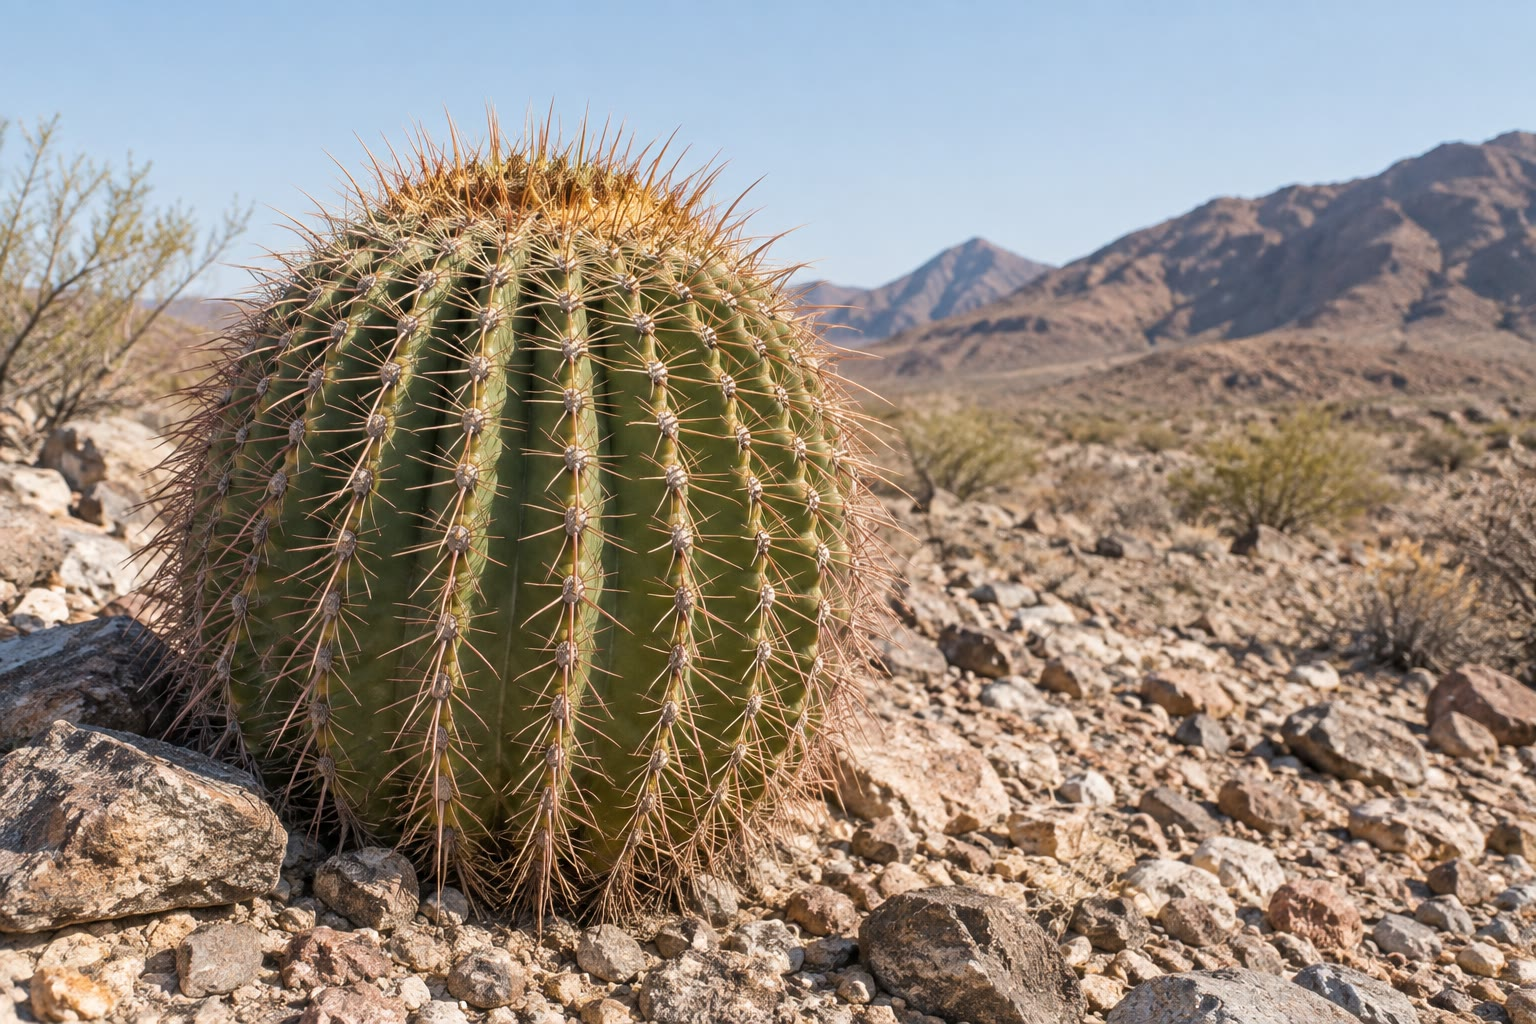
\includegraphics[width=0.55\linewidth]{images/book4/ai/b4-15-cactus.jpg}

{\small Een tonvormige cactus: een succulente stengel met een dikke
cuticula, ribben waardoor hij na regen kan opzwellen, bladeren teruggebracht
tot doorns, en huidmondjes die alleen 's nachts opengaan.}
\end{omfigure}

\section{Kou, zout en de stressrespons}

\begin{proposition}[Acclimatisatie aan stress]\label{prop:b2:plant-plasticity:stress}
\index{koudeacclimatisatie}\index{halofyt}\index{hitteschokeiwit}
Een week bij \qty{4}{\celsius} verlaagt de temperatuur waarbij winterrogge
sterft van \qty{-5}{\celsius} tot \qty{-25}{\celsius}: de cellen hebben
suikers en eiwitten opgestapeld die het vriespunt verlagen en membranen
beschermen, hun lipiden veranderd om vloeibaar te blijven, en
antivrieseiwitten gemaakt die de groei van ijskristallen tegenhouden; wat
doodt, is niet het ijs, dat zich onschadelijk tussen de cellen vormt, maar
de uitdroging van de cel doordat water haar verlaat om zich bij het ijs te
voegen. Enkele uren bij \qty{40}{\celsius} induceren
\emph{\omterm{prop:b2:plant-plasticity:stress}{hitteschokeiwitten}}, die gedenatureerde eiwitten opnieuw vouwen en de
cel bij \qty{45}{\celsius} beschermen. Zout wordt bestreden door uitsluiting
aan de wortel, opsluiting in de vacuole (met compatibele opgeloste stoffen
in het cytosol als tegenwicht) en, bij echte \emph{halofyten}, uitscheiding
via zoutklieren. De meeste van deze responsen verlopen via dezelfde
signalering: een sensor, een stijging van het cytosolische calcium,
\omterm{def:b2:plant-flowering:dormancy}{abscisinezuur}, en een reeks \omterm{prop:b2:cell-differentiation:transcriptional}{transcriptiefactoren} die honderden beschermende
genen aanschakelen --- een stressprogramma dat even algemeen is als de
immuunrespons van een dier, en daarmee vergelijkbaar ook kostbaar: de
geacclimatiseerde plant groeit langzaam, en een plant die acclimatiseert
wanneer dat niet nodig is, verliest het van een plant die dat niet doet.
\end{proposition}
\begin{proof}[Bewijsmateriaal]
Proeven met koudeacclimatisatie meten de temperatuur waarbij de helft van
de cellen van een blad sterft (de LT$_{50}$) vóór en na een periode bij lage
temperatuur; de verschuiving, van tien tot twintig graden in een week, wordt
door een week warmte ongedaan gemaakt. Mutanten die het koudeprogramma niet
kunnen aanschakelen (de \omterm{prop:b2:cell-differentiation:transcriptional}{CBF-transcriptiefactoren}), acclimatiseren slecht, en
planten die deze factoren constitutief tot expressie brengen, overleven
vorst zonder \omterm{def:b2:plant-plasticity:plasticity}{acclimatisatie} --- maar groeien als dwergen.
\end{proof}

\begin{omfigure}
\begin{tikzpicture}[every node/.style={font=\scriptsize}, >=stealth]
  \node[draw, rounded corners, fill=omExo!25, align=center] (s) at (0,0) {stress\\droogte, kou,\\zout, hitte};
  \node[draw, rounded corners, fill=omDef!15, align=center] (sen) at (3.2,0) {sensor\\(membraan, turgor,\\ontvouwen eiwitten)};
  \node[draw, rounded corners, fill=omDef!15, align=center] (ca) at (6.4,0) {secundaire boodschappers\\Ca$^{2+}$, ABA};
  \node[draw, rounded corners, fill=omProp!20, align=center] (tf) at (9.6,0) {transcriptie-\\factoren};
  \node[draw, rounded corners, fill=omThm!15, align=center] (out) at (12.8,0.9) {beschermende genen:\\opgeloste stoffen, antivries,\\chaperonnes, transporters};
  \node[draw, rounded corners, fill=omThm!15, align=center] (out2) at (12.8,-0.9) {vertraagde groei:\\de prijs};
  \draw[->, thick] (s) -- (sen); \draw[->, thick] (sen) -- (ca); \draw[->, thick] (ca) -- (tf);
  \draw[->, thick] (tf) -- (out); \draw[->, thick] (tf) -- (out2);
\end{tikzpicture}

{\small De gemeenschappelijke vorm van de stressrespons van een plant: een
sensor, een signaal van calcium en \omterm{def:b2:plant-flowering:dormancy}{abscisinezuur}, \omterm{prop:b2:cell-differentiation:transcriptional}{transcriptiefactoren}, en
een programma van beschermende genen --- betaald met groei.}
\end{omfigure}

\begin{example}[Signalen die liegen]\label{ex:b2:plant-plasticity:lie}
Plasticiteit is maar zo goed als het signaal. Een zaailing in de
verroodschaduw van een buur strekt zich --- terecht als die buur een
zaailing is die hij kan overgroeien; fataal als het een boom is, want de
reserves die aan stengel worden besteed, gaan verloren voor wortel en blad.
Dicht geplante gewassen beschaduwen elkaar, strekken zich en legeren;
veredelaars hebben tarwe en rijst geselecteerd die het verroodsignaal
negeren. Een warme week in februari laat bladeren uitlopen die een
maartvorst doodt; de planten die overleven, zijn die welke ook de kou tellen
(\cref{ch:b2:plant-flowering}). Elke plastische respons is een weddenschap
op de eerlijkheid van het signaal, en de \omterm{def:b2:plant-plasticity:plasticity}{reactienorm} wordt gevormd door hoe
vaak het signaal in het verleden van de lijn de waarheid sprak.
\end{example}

\section{Opgaven}

\begin{exercise}[$\star$]\label{exo:b2:plant-plasticity:1}
Definieer \omterm{def:b2:plant-plasticity:plasticity}{fenotypische plasticiteit}, \omterm{def:b2:plant-plasticity:plasticity}{reactienorm}, \omterm{def:b2:plant-plasticity:plasticity}{acclimatisatie} en
\omterm{def:b2:plant-plasticity:plasticity}{adaptatie}, met bij elk een voorbeeld uit de planten.
\end{exercise}

\begin{exercise}[$\star$]\label{exo:b2:plant-plasticity:2}
Beschrijf de vier behandelingen van coleoptielen door Darwin en wat elk ervan aantoonde.
\end{exercise}

\begin{exercise}[$\star$]\label{exo:b2:plant-plasticity:3}
Noem vijf verschillen tussen een \omterm{prop:b2:plant-plasticity:sunshade}{zonneblad} en een \omterm{prop:b2:plant-plasticity:sunshade}{schaduwblad}, en zeg
wanneer in het leven van het blad de keuze wordt gemaakt.
\end{exercise}

\begin{exercise}[$\star$]\label{exo:b2:plant-plasticity:4}
Hoe gaat een huidmondje open, wat opent het 's ochtends, en wat sluit het
bij droogte?
\end{exercise}

\begin{exercise}[$\star\star$]\label{exo:b2:plant-plasticity:5}
Bereken $\varphi$ voor $R{:}FR = 1.15$ (zon), $0.7$ (een open plek), $0.2$
(onder een bladerdak) en $0.05$ (diepe schaduw) met $a = 0.77$. Tussen welke
twee daarvan schakelt de plant de \omterm{thm:b2:plant-plasticity:phytochrome}{schaduwvermijding} aan als de drempel
$\varphi = 0.4$ is?
\end{exercise}

\begin{exercise}[$\star\star$]\label{exo:b2:plant-plasticity:6}
Een blad heeft $g_s = \qty{0.25}{mol.m^{-2}.s^{-1}}$, $w_i - w_a = 0.025$,
$c_a - c_i = \qty{100}{\micro mol/mol}$. Bereken $E$, $A$, de
watergebruiksefficiëntie in mol en in gram water per gram koolstof, en het
water dat per vierkante meter verloren gaat op een dag van 12 uur.
\end{exercise}

\begin{exercise}[$\star\star$]\label{exo:b2:plant-plasticity:7}
Bereken de vorige opgave opnieuw voor een \omterm{prop:b2:plant-plasticity:xerophytes}{CAM-plant} waarvan de huidmondjes
's nachts opengaan, met $w_i - w_a = 0.005$ en dezelfde geleidbaarheid. Met
welke factor dalen de waterkosten van koolstof?
\end{exercise}

\begin{exercise}[$\star\star$]\label{exo:b2:plant-plasticity:8}
Een statoliet is een zetmeelkorrel met straal \qty{2}{\micro m} en dichtheid
\qty{1500}{kg/m^3} in cytoplasma met dichtheid \qty{1100}{kg/m^3} en
viscositeit \qty{0.01}{Pa.s}. Bereken zijn zinksnelheid (Stokes) en de tijd
om een cel van \qty{10}{\micro m} over te steken. Waarom heft een klinostaat
die één keer per minuut draait de gravitropie op?
\end{exercise}

\begin{exercise}[$\star\star$]\label{exo:b2:plant-plasticity:9}
Een stengel van \qty{2}{mm} dik groeit \qty{2}{\%} per uur over een zone van
\qty{20}{mm}. Licht van één kant verdeelt de auxine als $60 : 40$.
Over welke hoek is hij na twee uur gebogen? Na hoelang staat hij onder
\qty{90}{\degree} ten opzichte van zijn oorspronkelijke richting?
\end{exercise}

\begin{exercise}[$\star\star\star$]\label{exo:b2:plant-plasticity:10}
Een zaailing met \qty{50}{mg} reserves strekt zich in het open veld met
\qty{2}{cm} per dag en onder een bladerdak met \qty{4}{cm} per dag, en
besteedt per centimeter stengel \qty{1}{mg} reserves bovenop wat zijn
bladeren leveren. Het bladerdak ligt \qty{30}{cm} boven hem in een
brandnetelveld en \qty{10}{m} in een bos. In welk geval slaagt de
\omterm{thm:b2:plant-plasticity:phytochrome}{schaduwvermijding}, en wat gebeurt er in het andere?
\end{exercise}

\begin{exercise}[$\star\star\star$]\label{exo:b2:plant-plasticity:11}
Leg uit waarom bevriezing een cel doodt door uitdroging en niet door ijs, wat
een week kou doet om dat te voorkomen, en waarom een plant die het
koudeprogramma het hele jaar tot expressie brengt, een dwerg is.
\end{exercise}

\begin{exercise}[$\star\star\star$]\label{exo:b2:plant-plasticity:12}
``Plasticiteit is een weddenschap op de eerlijkheid van een signaal.''
Bespreek dit aan de hand van het verroodsignaal, de warme week in februari,
en het veredelen van gewassen die hun buren negeren.
\end{exercise}

\section{Vraagstuk: een zaailing onder het bladerdak}

\begin{problem}[{Weekendvraagstuk --- het lichtklimaat, de strekking, de
waterbalans en de tropieën van een zaailing, berekend uit de fysica van zijn
sensoren, met als besluit de toestand van zijn fytochroom, zijn hoogte na
twee weken en zijn dagelijkse waterverbruik}]
\label{pb:b2:plant-plasticity:1}
Een berkenzaailing kiemt onder een bladerdak dat \qty{3}{\%} van het
zonlicht doorlaat en $R{:}FR$ verlaagt van $1.15$ tot $0.2$
($a = 0.77$). In de volle zon zou hij zich met \qty{1.5}{cm} per dag
strekken; onder het bladerdak wordt zijn strekkingssnelheid vermenigvuldigd
met $1 +
2(0.6 - \varphi)$. Zijn stengel is \qty{2}{mm} dik met een groeizone van
\qty{15}{mm}. Bladeren: \qty{20}{cm^2} in totaal; $g_s =
\qty{0.2}{mol.m^{-2}.s^{-1}}$; $w_i - w_a = 0.015$ in de schaduw,
$0.03$ op een open plek; $c_a - c_i = \qty{80}{\micro mol/mol}$; de dag
duurt \qty{14}{h}. Statolieten: straal \qty{2.5}{\micro m}, dichtheid
\qty{1500}{kg/m^3}, in cytoplasma van \qty{1100}{kg/m^3} en
\qty{0.01}{Pa.s}.

\medskip
\noindent\textbf{Deel I --- Het licht.}
\begin{enumerate}
  \item Bereken $\varphi$ in het open veld en onder het bladerdak.
  \item Wat concludeert de zaailing uit $\varphi$, en wat zou hij
        concluderen als het bladerdak \qty{3}{\%} van het licht doorliet
        zonder de kleur ervan te veranderen (een schaduwdoek)?
  \item Bereken de strekkingssnelheid onder het bladerdak.
  \item Hoe hoog is de zaailing daar na 14 dagen, tegenover een broertje in
        het open veld?
  \item Aan één kant ontstaat een open plek, waardoor $R{:}FR$ aan die kant
        stijgt tot
        $0.8$. Welke twee responsen volgen, en via welke twee
        fotoreceptoren?
  \item Waarom zijn bladeren die onder het bladerdak zijn ontwikkeld groter
        en dunner, en wat gebeurt er met ze als het bladerdak wordt gekapt?
\end{enumerate}

\medskip
\noindent\textbf{Deel II --- Buigen naar de open plek.}
\begin{enumerate}[resume]
  \item Licht uit de open plek verdeelt de auxine over de stengel als
        $65 : 35$. Bereken met de strekkingssnelheid onder het bladerdak
        uit vraag 3 de relatieve verlenging van elke kant van de groeizone
        in één uur.
  \item Bereken de hoek waarover de stengel na één uur is gebogen.
  \item Na hoelang wijst de stengel recht naar de open plek, als die onder
        \qty{60}{\degree} van de verticaal ligt?
  \item De stengel helt nu over. Bereken de zinksnelheid van een statoliet
        en de tijd om een cel van \qty{12}{\micro m} over te steken.
  \item De gravitropie en de fototropie van de scheut zijn het nu oneens.
        Welke wint bij een plant die schaduw vermijdt, en waarom is dat
        adaptief?
  \item Een wortel van dezelfde zaailing wordt door een steen
        \qty{45}{\degree} gekanteld. Voorspel zijn respons en leg uit waarom
        die tegengesteld is aan die van de scheut, hoewel het mechanisme
        hetzelfde is.
\end{enumerate}

\medskip
\noindent\textbf{Deel III --- Water.}
\begin{enumerate}[resume]
  \item Bereken de transpiratie per vierkante meter in de schaduw, en het
        water dat de bladeren van de zaailing per dag verliezen.
  \item Bereken de vastgelegde koolstof per vierkante meter per seconde en
        per dag, en de watergebruiksefficiëntie in gram water per gram
        koolstof.
  \item Wat is de totale dagelijkse koolstofwinst van de zaailing in de
        schaduw, in milligram?
  \item Bereken het waterverlies en de efficiëntie opnieuw op de open plek.
  \item De bodem droogt uit en \omterm{def:b2:plant-flowering:dormancy}{abscisinezuur} verlaagt $g_s$ tot
        \qty{0.02}{mol.m^{-2}.s^{-1}}. Bereken $E$ en $A$ opnieuw (neem aan
        dat $c_a - c_i$ stijgt tot \qty{200}{\micro mol/mol}). Welke daalt
        het meest, en waarom?
  \item De zaailing heeft \qty{5}{g} bladweefsel dat voor \qty{85}{\%} uit
        water bestaat en een vijfde daarvan kan verliezen voordat het
        verwelkt. Hoelang houdt hij het op de open plek uit met open
        huidmondjes als de wortels niets aanvoeren?
  \item Leg uit waarom een CAM-strategie niet zou passen bij een
        berkenzaailing onder een bladerdak.
\end{enumerate}

\medskip
\noindent\textbf{Deel IV --- De weddenschap.}
\begin{enumerate}[resume]
  \item De zaailing heeft \qty{100}{mg} reserves en besteedt in de schaduw
        \qty{2}{mg} per centimeter stengel bovenop wat zijn bladeren
        leveren. Hoeveel stengel kan hij op reserves alleen bouwen?
  \item Het bladerdak is een brandnetelveld \qty{40}{cm} boven hem; daarna
        een bos \qty{8}{m} boven hem. Zeg in elk geval of de strekking het
        licht bereikt voordat de reserves op zijn, en wat in het bos de betere
        respons zou zijn geweest.
  \item Een berk is een pionier van open grond; een beukenzaailing kan
        decennialang in diepe schaduw wachten. Vergelijk hun te verwachten
        \omterm{def:b2:plant-plasticity:plasticity}{reactienormen} ten opzichte van $\varphi$.
  \item Een plantenveredelaar wil een dicht geplant gewas dat zich niet
        strekt. Welke sensor of respons zou je uitschakelen, en welk
        neveneffect moet je controleren?
  \item Leg in twee zinnen uit waarom een plant die haar buren niet kan
        waarnemen en een plant die ze altijd gelooft, allebei slechter af
        zijn dan een plant die ze soms gelooft.
  \item Formuleer het resultaat: $\varphi$ in zon en schaduw, de hoogte van
        de zaailing na 14 dagen, en zijn dagelijkse waterverbruik in de
        schaduw en op de open plek.
\end{enumerate}
\end{problem}
